\documentclass[a4paper, 12pt]{book}
\usepackage{graphicx}
\usepackage[french]{babel}
\usepackage[utf8]{inputenc}
\usepackage[T1]{fontenc}
\usepackage{multirow}
\usepackage{listings}
\usepackage{float}
\usepackage{url}
\usepackage[french]{algorithm}
\usepackage{style/myalgorithm}
\usepackage{amsmath,amsfonts,amssymb}
\newcommand{\fBm}{\emph{fBm}~}
\newcommand{\etal}{\emph{et al.}~}
\newcommand{\glAd}{\emph{GL4D}~}
\newcommand{\apiopengl}{API OpenGL\textsuperscript{\textregistered}~}
\newcommand{\opengl}{OpenGL\textsuperscript{\textregistered}~}
\newcommand{\opengles}{OpenGL\textsuperscript{\textregistered}ES~}
\newcommand{\clang}{langage \texttt{C}}
\newcommand{\codesource}{\textsc{Code source}~}
\floatstyle{ruled}
\newfloat{programslist}{htbp}{locs}
\newcommand{\listofprograms}{\listof{programslist}{Liste des codes source}}
\newcounter{program}[subsection]
\renewcommand{\theprogram}{\arabic{chapter}.\arabic{program}}


\newenvironment{program}[1]{
  \if\relax\detokenize{#1}\relax
  \gdef\mycaption{\relax}
  \else
  \gdef\mycaption{#1}
  \fi
  \refstepcounter{program}
  \addcontentsline{locs}{section}{#1}
  \footnotesize
}{
  \begin{description}
    \item[\codesource \theprogram]--~\mycaption
  \end{description}
}
\setcounter{secnumdepth}{3}
\setcounter{tocdepth}{3}

\begin{document}
\begin{titlepage}
  \begin{center}
    \begin{tabular*}{\textwidth}{l@{\extracolsep{\fill}}r}
      
\includegraphics[height=2cm]{images/m2ise.png}&
      
\includegraphics[height=2.5cm]{images/p8.png}
    \end{tabular*}
    \small 
    \rule{\textwidth}{.5pt}~\\
    \large 
    \textsc{Université Paris 8 - Vincennes à Saint-Denis}\vspace{0.5cm}\\
    \textbf{Master 2 : Informatique des Systèmes Embarqués}\vspace{3.0cm}\\
    \Large
    \textbf{Reconnaissance automatique de la parole}\vspace{1.5cm}\\
    \large
    Amar \textsc{Bessalah}\\
    {\&}\\
    Mohamed \textsc{Benomari}\vspace{1.5cm}\\
    Date de rendu : le 03/07/2020\vspace{2cm}\\
  \end{center}\vspace{2cm}~\\
  \begin{tabular}{ll}
    \hspace{-0.45cm}Tuteur~:~&~Sami \textsc{Boutamine}\\
  \end{tabular}
\end{titlepage}
\frontmatter
\chapter*{Résumé}
\markboth{\sc Résumé}{}
\addcontentsline{toc}{chapter}{Résumé} 

Ce document regroupe les informations nécessaires à la compréhension et à la mise en place de certaines méthodes dîtes de reconnaissance de la parole. En outre, il sera question des outils de traitement de la parole existants, dont certains que nous devrons apprendre à maîtriser afin de développer notre programme.\\

Le projet en question repose sur le développement d'un programme informatique qui devra permettre l'identification d'une personne à partir de sa voix. Avant d'en arriver là, le programme devra d'abord effectuer un traitement de la voix de cette personne, afin d'en obtenir un modèle qui sera utilisé pour comparer cette voix avec des voix diverses de test, puis générer un résultat nous permettant de savoir si les deux voix correspondent, et donc si il s'agit de la même personne ou non.\\

Nous entamerons ce rapport par une présentation des techniques permettant l'acquisition du son et son traitement. Puis, nous parlerons des méthodes permettant d'extraire les caractéristiques d'un son. Ensuite, nous aborderons les techniques permettant l'entraînement des modèles. Enfin, nous décrirons les méthodes utilisées pour tester l'identification d'une personne et nous analyserons les résultats obtenus. 

%% Table des matières
\tableofcontents
%% La liste des figure est optionnelle (si votre rapport manque de
%% contenu ajouter ce type de pages sera perçu négativement)
\listoffigures
%% La liste des programmes est optionnelle (si votre rapport manque de
%% contenu ajouter ce type de pages sera perçu négativement)
%\listofprograms
\mainmatter
\chapter*{Introduction}
\markboth{\sc Introduction}{}
\addcontentsline{toc}{chapter}{Introduction}

Le domaine de la reconnaissance vocale se compose d'une multitude de méthodes et de techniques permettant d'effectuer des traitements de la parole. 

Parmi ces techniques, nous retrouvons notamment la reconnaissance du locuteur (permet d'identifier une personne d'après sa voix), la reconnaissance de la parole (permet d'analyser une voix afin de la transcrire sous forme de texte), ou encore la synthèse de la parole (permet de créer une parole artificielle à partir d'un texte).

De nos jours, ces techniques sont très répandues dans les outils informatiques de tous les jours (ordinateurs, smartphones, objets connectés, etc), généralement pour la vérification d'identité ou encore l'exécution de commandes vocales. Ces plateformes offrent une utilisation simple et rapide de ces techniques, tout en restant performantes.\\

Afin de tester les capacités et les performances de certaines de ces techniques, nous allons travailler sur un projet de reconnaissance de locuteur, qui devra permettre d'identifier une personne d'après sa voix.

L'objectif final étant de pouvoir répondre à la question \guillemotleft{}~Qui parle ?~\guillemotright{}.\\

Nous allons nous appuyer sur les nombreux outils développés dans le but de faciliter le traitement de la parole, et ainsi réaliser notre propre programme d'identification de locuteur.

% chapitre 1 section 1 : ############################################

\chapter{État de l'art}

\section{Acquisition du son}

Une membrane vibre sous l'effet de la pression acoustique et un dispositif qui dépend de la technologie du microphone convertit ces oscillations en signaux électriques. La conception d'un microphone comporte une partie acoustique et une partie électrique, qui vont définir ses caractéristiques et le type d'utilisation (https://fr.wikipedia.org/wiki/Microphone).

\subsection{Type de microphone}

Le choix du microphone dépend des applications de notre modèle de reconnaissance, dans le cas ou nous favorisons une source émettrice lointaine ou proche, avec beaucoup de bruit ou peu. 


\subsubsection{Microphones dynamiques}

Les microphones dynamiques utilisent un ensemble diaphragme / bobine acoustique / aimant qui forme un générateur électrique miniature piloté par le son. Les ondes sonores frappent une fine membrane de plastique (diaphragme) qui vibre en réponse. Une petite bobine de fil (bobine mobile) est fixée à l'arrière du diaphragme et vibre avec ce dernier. La bobine acoustique elle-même est entourée d'un champ magnétique créé par un petit aimant permanent. C'est le mouvement de la bobine acoustique dans ce champ magnétique qui génère le signal électrique correspondant au son capté par un microphone dynamique. Les microphones dynamiques ont une construction relativement simple et sont donc économiques et robustes. Ils peuvent fournir une excellente qualité sonore et de bonnes spécifications dans tous les domaines de la performance du microphone. En particulier, ils peuvent gérer des niveaux sonores extrêmement élevés: il est presque impossible de surcharger un microphone dynamique. De plus, les microphones dynamiques sont relativement peu affectés par les extrêmes de température et d'humidité. La dynamique est le type le plus utilisé dans le renforcement acoustique général.


\subsubsection{Microphones à condensateur}

Les microphones à condensateur sont basés sur un assemblage diaphragme / plaque arrière chargé électriquement qui forme un condensateur sensible au son. Ici, les ondes sonores font vibrer un diaphragme très fin en métal ou en plastique recouvert de métal. Le diaphragme est monté juste devant une plaque arrière en métal rigide ou en céramique revêtue de métal. 

En terme électrique, cet ensemble ou élément est appelé un condensateur (appelé historiquement un \guillemotleft{}~condensateur~\guillemotright{}), qui a la capacité de stocker une charge ou une tension. Lorsque l'élément est chargé, un champ électrique est créé entre le diaphragme et la plaque arrière, proportionnel à leur espacement. C'est la variation de cet espacement, due au mouvement du diaphragme par rapport à la plaque arrière, qui produit le signal électrique correspondant au son capté par un microphone à condensateur. La construction d'un microphone à condensateur doit inclure une disposition permettant de maintenir la charge électrique ou la tension de polarisation. Un microphone à condensateur électret a une charge permanente, maintenue par un matériau spécial déposé sur la plaque arrière ou sur le diaphragme. Les types non-électriques sont chargés (polarisés) au moyen d'une source d'alimentation externe. La majorité des microphones à condensateur pour l'amplification du son sont du type électret. Tous les condenseurs contiennent des circuits actifs supplémentaires, permettant à la sortie électrique de l'élément d'être utilisée avec des entrées de microphone classiques. 

Cela nécessite que tous les microphones à condensateur soient alimentés: soit par piles, soit par alimentation fantôme (méthode consistant à alimenter un microphone par le câble du microphone lui-même). Les microphones à condensateur présentent deux limitations potentielles dues aux circuits supplémentaires: premièrement, les composants électroniques produisent une faible quantité de bruit; deuxièmement, il existe une limite au niveau de signal maximal que l'électronique peut gérer. Pour cette raison, les spécifications du microphone à condensateur incluent toujours un facteur de bruit et un niveau sonore maximal. Les bonnes conceptions, cependant, ont des niveaux de bruit très bas et sont également capables de très grande plage dynamique.

\subsubsection{Différence entre microphones à condensateur et microphone dynamique}

Les microphones à condensateur sont plus complexes que les dynamiques et ont tendance à être un peu plus coûteux. De plus, les condenseurs peuvent être affectés par des températures et des taux d'humidité extrêmes, ce qui peut les rendre bruyants ou en panne de façon temporaire. Cependant, les condenseurs peuvent facilement être fabriqués avec une sensibilité plus élevée et peuvent fournir un son plus doux et plus naturel, en particulier à des fréquences élevées. La réponse en fréquence plate et la plage de fréquence étendue sont beaucoup plus faciles à obtenir dans un condenseur. De plus, les microphones à condensateur peuvent être très petits sans perte significative de performances. Image Microphone à condensateur La décision d'utiliser un microphone à condensateur ou dynamique dépend non seulement de la source sonore et du système de renforcement acoustique, mais également du réglage physique. D'un point de vue pratique, si le microphone doit être utilisé dans un environnement sévère tel qu'un club de rock'n'roll ou pour le son en extérieur, des types dynamiques constitueront un bon choix. Dans un environnement plus contrôlé, tel qu'une salle de concert ou une configuration théâtrale, un microphone à condensateur peut être préféré pour de nombreuses sources sonores, en particulier lorsque la qualité sonore optimale est désirée (https://www.shure.com/en-US/support/find-an-answer/difference-between-a-dynamic-andcondenser-microphone)

\subsection{Étapes de traitement du son}

Le traitement numérique du signal par ordinateur exige que le signal soit converti en une suite de nombres (numérisation). Cette conversion se décompose, sur le plan théorique, en trois opérations

\begin{figure}[htbp]
  \centering
  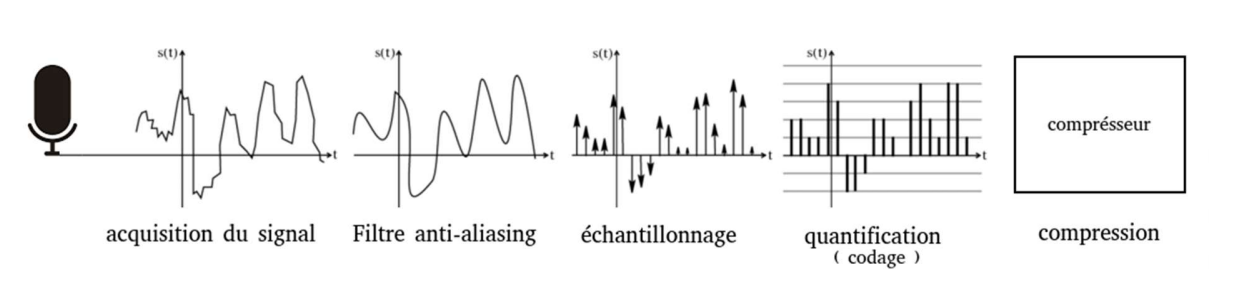
\includegraphics[width=1.2\linewidth]{fig/etape-acquisition-son.png}
  \caption{Étapes de traitement du son}
\end{figure}

\subsubsection{Échantillonnage}

L'échantillonnage consiste à prélever les valeurs d'un signal à intervalles définis, généralement réguliers. Il produit une suite de valeurs discrètes nommées échantillons \texttt{(https://fr.wikipedia.org/wiki/\%C3\%89chantillonnage\_(signal))}.\\

\textbf{Cadence d'échantillonnage (théorème de Shannon-Nyquist) :}

Si toutes les fréquences du signal sont inférieures à la moitié de la fréquence d'échantillonnage, il peut être parfaitement reconstitué (fréquence d'échantillonnage = 2x frequenceMax du signal).

\subsubsection{Quantification (conversion analogique numérique)}
En traitement des signaux, la quantification est le procédé qui permet d'approcher un signal continu par les valeurs d'un ensemble discret d'assez petite taille. L'amplitude relevée à chaque étape d'échantillonnage va être codée en binaire sur un certain nombre de bits : 8, 16, 24, 32, etc. C'est la quantification. Là encore, plus le nombre de bits va être élevé, plus la valeur numérique de l'amplitude sera proche de la valeur originale.

\subsubsection{Compression}
La compression audio est une forme de compression de données qui a pour but de réduire la taille d'un flux audio numérique en vue d'une transmission (contraintes de largeur de bande et de débit) ou d'un stockage (contrainte d'espace de stockage). On distingue la compression sans perte, qui permet de reconstituer exactement les données d'origine, de la compression en général, « avec pertes », qui abandonne des données jugées non nécessaires à l'écoute, au profit de la diminution du débit ou de la taille des fichiers. 


% chapitre 1  section 2: ############################################

\section{Extraction de paramètres}

Une fois l'enregistrement audio effectué, il sera traité afin d'obtenir des données utilisables par un programme informatique (conversion d'un signal analogique vers un signal numérique/digital).

\subsection{Reconnaissance vocale : paramétrisation / traitement}

Le traitement de l'enregistrement obtenu passe par l'analyse de plusieurs paramètres qui le composent (volume sonore, bruits de fond, intonation, etc), appelés traits prosodiques. Les différents traits prosodiques (paramètres prosodiques) :

\begin{itemize}
    \item l'accent 
    \item le ton 
    \item l'intonation 
    \item la jointure (ex : \guillemotleft{}~coopérer~\guillemotright{}) 
    \item la pause 
    \item le rythme
    \item le tempo et le débit
\end{itemize}

Ces caractéristiques vont influer sur la manière dont certains sons vont être interprétés par le programme de reconnaissance vocale.

\subsection{Algorithmes de traitement du signal audio}

Afin de traiter le signal audio, il lui sera appliqué un algorithme spécifiquement crée pour ce type de signal. Il en existe plusieurs, certains plus efficaces selon la clarté de l'enregistrement, la présence de bruit, etc. Le signal ne sera pas traiter en un seul bloc, mais sera découpé en plusieurs segments (selon un intervalle de temps ou selon un intervalle de sons) de même longueur (environ 20 à 25 millisecondes) et qui se superposeront (la fin d'un segment – les 10 dernières millisecondes – et le début du segment suivant – les 10 premières millisecondes – seront à cheval sur les mêmes données). De cette manière, nous pouvons travailler sur des échantillons de sons plus petits et obtenir un résultat plus précis après traitement.

\subsubsection{Transformation de Fourier}

C'est l'une des opération les plus fréquemment effectuée pour le traitement des signaux. Elle permet de passer de la représentation temporelle d'un signal à sa représentation fréquentielle / spectrale.

\begin{figure}[htbp]
  \centering
  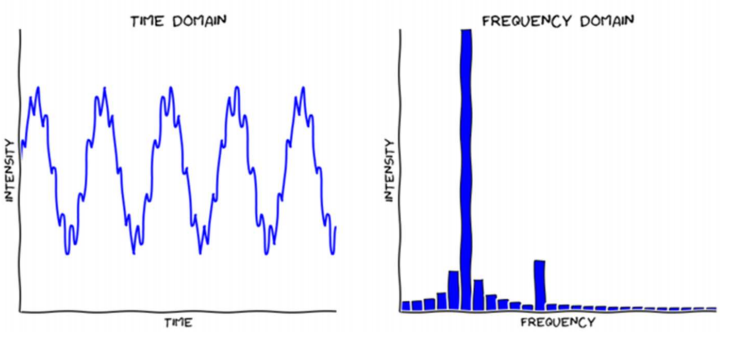
\includegraphics[width=1\linewidth]{fig/fourier.png}
  \caption{Transformation d'un signal}
\end{figure}

\subsubsection{Transformation de Fourier discrète}

La transformation de Fourier discrète (TFD ou DFT en anglais) est un outil mathématique de traitement du signal numérique, qui est l'équivalent discret de la transformation de Fourier continue qui est utilisée pour le traitement du signal analogique. Elle est typiquement utilisée sur des sons.

\subsubsection{Codage prédictif linéaire (LPC – Linear Predictive Coding)}

Le codage prédictif linéaire est une méthode de codage et de représentation de la parole. Elle est appliquée sur un signal, afin d'en obtenir un modèle.

« Elle repose principalement sur l'hypothèse que la parole peut être modélisée par un processus linéaire. Il s'agit donc de prédire le signal à un instant n à partir des p échantillons précédents. La parole n'étant cependant pas un processus parfaitement linéaire, la moyenne que constitue la somme pondérée du signal sur p pas de temps introduit une erreur qu'il est nécessaire de corriger par l'introduction du terme e(n).

\subsubsection{MFCC - Mel Frequency Cepstral Coefficients}

Le MFCC permet d'appliquer des transformations à un signal (semblables à une transformation de Fourier), afin d'en obtenir une modélisation sous forme d'un spectre. C'est actuellement le plus utilisé pour les programmes de reconnaissance vocale.

Son avantage est qu'il utilise l'échelle de Mel pour mesurer la fréquence d'un signal, ainsi,
son spectre sera plus précis et aura un aspect très proche de ce qui serait perçu par un humain.

\begin{figure}[htbp]
  \centering
  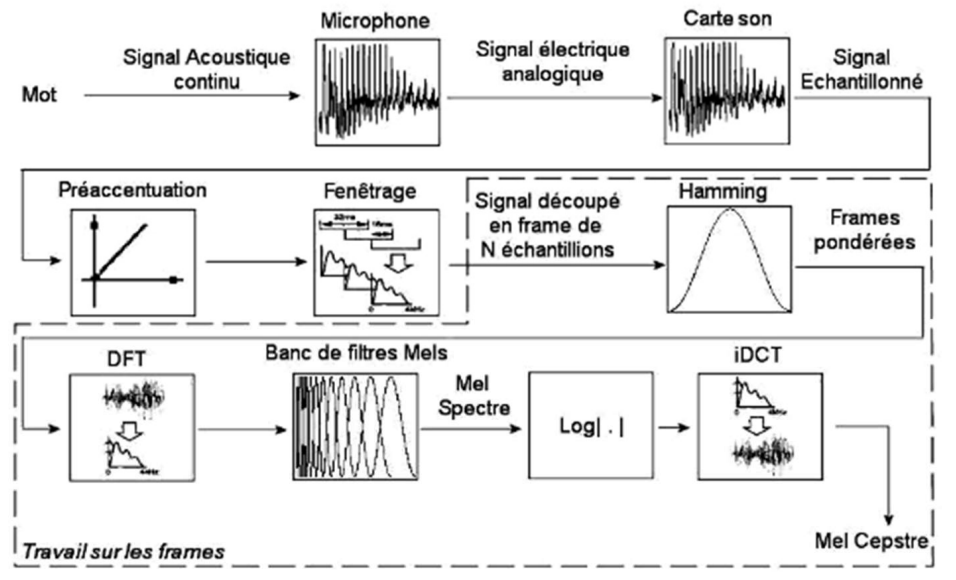
\includegraphics[width=1\linewidth]{fig/mfcc.png}
  \caption{Étapes du calcul des coefficients MFCC}
\end{figure}


\textbf{Efficacité de MFCC :}

MFCC est considéré comme très efficace lorsqu'il est appliqué sur un enregistrement propre (pas de bruits de fond, bon volume vocal, etc), mais moins robuste lors de présence de bruit.

On notera néanmoins que l'analyse MFCC Aurora a été développée de manière à effectuer un dé-bruitage sur un tel signal.

%\textbf{Exemple de mise en place}

%(page 16) : https://hal.inria.fr/tel-01251128/document

\textbf{Résultat :}

Le spectre finalement obtenu représente ainsi les informations phonétiques citées précédemment (traits prosodiques). Nous pouvons alors utiliser les valeurs de ce spectre afin d'effectuer les opérations voulues (modification du signal, récupération d'un d'un son, etc).

\subsection{Outils d'extraction des features}

\subsubsection{SPro}

SPro est une boîte à outils de traitement du signal vocal gratuit qui fournit des commandes d'exécution implémentant des algorithmes d'extraction de fonctionnalités standard pour les applications liées à la parole et une bibliothèque C pour implémenter de nouveaux algorithmes et utiliser des fichiers SPro dans vos propres programmes.

SPro fournit des techniques d'extraction de fonctionnalités utilisées dans les applications vocales. Il existe des commandes pour les représentations suivantes:
énergies de banc de filtres
coefficients cepstraux
représentation dérivée de prédiction linéaire


\begin{enumerate}
  \item filter-bank energies
  \item cepstral coefficients
  \item linear prediction derived representation
\end{enumerate} 


\subsubsection{Htk}

HTK est une boîte à outils portable pour la construction et la manipulation de modèles de Markov cachés il se compose d'un ensemble de modules de bibliothèque et d'outils disponibles sous forme de source C. Les outils fournissent des installations sophistiquées pour l'analyse de la parole. HTK est principalement utilisé pour la recherche sur la reconnaissance vocale, bien qu'il ait été utilisé pour de nombreuses autres applications, notamment la recherche sur la synthèse vocale, la reconnaissance de caractères et le séquençage d'ADN

% chapitre 1 section 3 : ############################################

\section{Apprentissage du modéle}

Dans cette étape on réalise une association entre les segments élémentaires de la parole et les éléments lexicaux. Cette association fait appel à une modélisation statistique ou par réseaux de neurones artificiels ou par algorithme de déformation temporelle dynamique

\subsection{Approche statistique}

L'RAS vise à convertir le signal vocal en texte et ce processus peut être formulé statistiquement comme suit. Soit un ensemble d'observations acoustiques O = (o1, o2, o3, on) (séquence de vecteurs de parole, où oi est le vecteur de parole observé à l'instant i), qui est la séquence de mots W = (w1, w2, Wn) qui a la probabilité maximale


\begin{figure}[htbp]
  \centering
  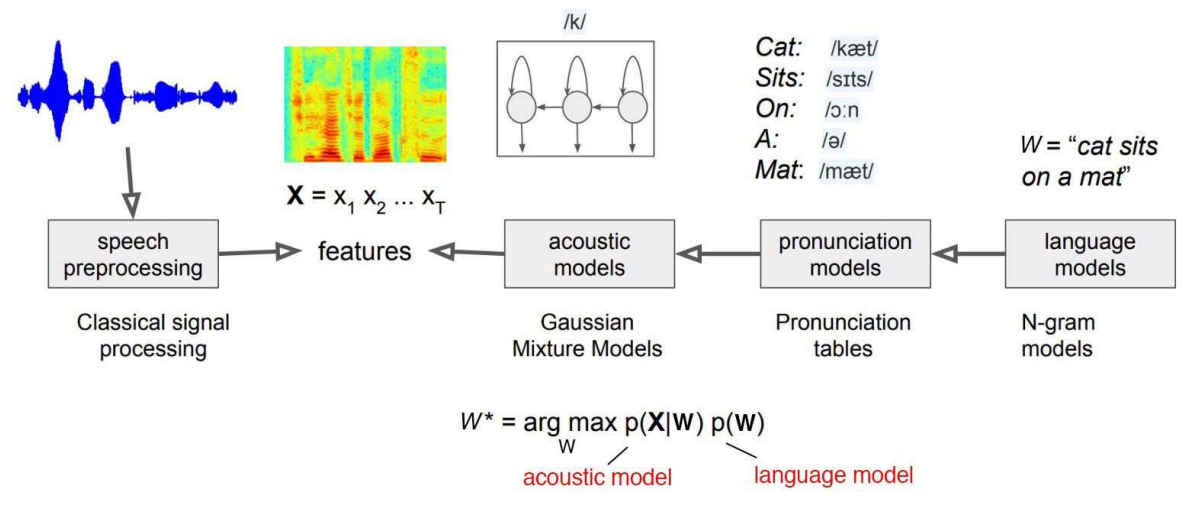
\includegraphics[width=1\linewidth]{fig/model.png}
  \caption{Etape modéle statistique}
\end{figure}

\subsubsection{Modèle de langue}

Le modèle de langue décide si un mot (ou une phrase) est valide dans une langue donnée Un modèle de langage statistique est une distribution de probabilité sur des séquences de mots. Étant donné une telle séquence, disons de longueur m, il attribue une probabilité à la séquence entière.

\textbf{Unigram}

Un modèle unigramme peut être traité comme la combinaison de plusieurs automates finis à un état. [1] Il divise les probabilités de différents termes dans un contexte.

Dans ce modèle, la probabilité de chaque mot dépend uniquement de la probabilité de ce mot dans le document, de sorte que nous avons uniquement des automates finis à un état en tant qu'unités. L'automate lui-même a une distribution de probabilité sur tout le vocabulaire du modèle, en faisant un total de 1. Ce qui suit est une illustration du modèle unigramme d'un document.


\textbf{n-gram}

Dans un modèle à n-grammes on cherche la probabilité P (w1, w2, wm) d'observer la phrase w1, w2, wm

On suppose que la probabilité d'observer le i-ème mot wi dans l'historique de contexte des mots i-1 précédents peut être approximée par la probabilité de l'observer dans l'historique de contexte raccourci des n-1 mots précédents (propriété de Markov d'ordre n) .

La probabilité conditionnelle peut être calculée à partir des comptes de fréquence du modèle ngramme


Les termes modèles de langage bigram et trigram désignent les modèles à n-grammes avec n = 2 et n = 3, respectivement.

\textbf{Exponential}

Les modèles de langage d'entropie maximum cherche à coder la relation entre un mot et l'historique ngram à l'aide de fonctions.

\textbf{Neural network}

La probabilité d'une séquence de mots peut être obtenue à partir de la probabilité de chaque mot étant donné le contexte des mots qui le précèdent, en utilisant la règle de probabilité en chaîne (une conséquence du théorème de Bayes)

La plupart des modèles de langage probabilistes (y compris les modèles de langage réseau neuronal publiés) approchent la probabilité en utlisant un contexte fixe de taille n - 1, c'est-à-dire en utilisant <eq9>, comme en n-grammes.

Dans le modèle introduit dans (Bengio et al 2001, Bengio et al 2003), la prédiction probabiliste <eq10> est obtenue comme suit. Tout d'abord, chaque mot wt - i (représenté par un entier dans [1, N]) dans le contexte de n-1 mot est mappé sur un vecteur de caractéristique ddimensionnel associé Cwt - i, qui est la colonne wt - i de la matrice de paramètres C. Le vecteur Ck contient les fonctions apprises pour le mot k. 



\subsubsection{Modéle acoustique}

Le modèle acoustique doit estimer la probabilité de prononcer un message, à partir d'une séquence de mots.

Pour tout w donné, le modèle acoustique correspondant est synthétisé en concaténant des modèles de téléphone pour créer des mots tels que définis par un dictionnaire de prononciation.

Un modèle acoustique est utilisé dans la reconnaissance automatique de la parole pour représenter la relation entre un signal audio et les phonèmes ou autres unités linguistiques qui composent la parole. Le modèle est appris à partir d'un ensemble d'enregistrements audio et de leurs transcriptions correspondantes. Il est créé en prenant des enregistrements audio de la parole et leurs transcriptions de texte, et en utilisant un logiciel pour créer des représentations statistiques des sons qui composent chaque mot.

\textbf{HMM ( hidden markov model )}

Une chaîne de Markov contient tous les états possibles d'un système et la probabilité de passer d'un état à un autre.

\begin{figure}[htbp]
  \centering
  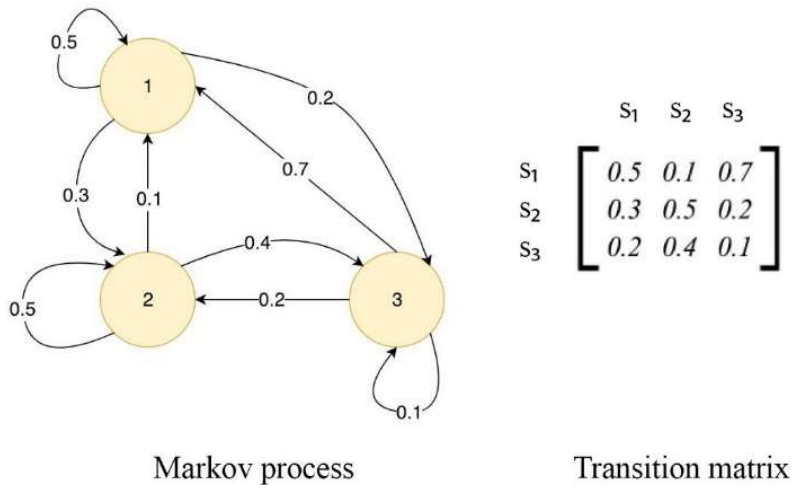
\includegraphics[width=0.7\linewidth]{fig/markov.png}
  \caption{Chaîne de Markov}
\end{figure}


Ce modèle sera beaucoup plus facile à manipuler. Cependant, dans de nombreux systèmes ML, tous les états ne sont pas observables et nous appelons ces états états cachés ou états internes. Certains peuvent les traiter comme des facteurs latents pour les intrants. Par exemple, il peut être difficile de savoir si je suis heureuse ou triste. Mon état interne sera {H ou S}. Mais nous pouvons obtenir des indications de ce que nous observons. Par exemple, lorsque je suis heureux, j'ai 0,2 chance de regarder un film, mais quand je suis triste, cette chance monte à 0,4. La probabilité d'observer un observable étant donné un état interne s'appelle la probabilité d'émission. La probabilité de passer d'un état interne à un autre s'appelle la probabilité de transition. Les modèles acoustiques les plus utilisés sont :


\begin{enumerate}

\item Modéle acoustique HMM/GMM
\item Modéle acoustique HMM/DNN

\end{enumerate}


\subsection{Approche par réseau de neurones}

L'approche à base de réseau de neurones consiste à mettre en place un modèle de bout en bout qui englobe de plus en plus de composants dans le pipeline de l'approche statistique. Les 2 plus populaires sont (1) la classification temporelle connexionniste (CTC), qui est largement utilisée de nos jours chez Baidu et Google, mais elle nécessite beaucoup de training ; et (2) séquence à séquence (Seq-2-Seq), qui ne nécessite pas de personnalisation manuelle.
La motivation de base est que nous voulons faire de la reconnaissance vocale de bout en bout. On nous donne l'audio X - qui est une séquence d'images de x1 à xT, et le texte de sortie correspondant Y - qui est une séquence de y1 à yL. Y est juste une séquence de texte (transcription) et X est le spectrogramme traité audio. Nous voulons effectuer la reconnaissance vocale en apprenant un modèle probabiliste p (Y | X): en commençant par les données et en prédisant les séquences cibles elles-mêmes.


\subsection{Approche par Dynamic time wrapping approch(DTW)}
DTW est une méthode pour mesurer la similitude d'un modèle avec différents amplitude. Plus la distance produite est petite, plus les deux motifs sonores sont similaires. Les deux modèles sonores sont similaires, donc les deux voix sont censées être les mêmes. Les données initiales sur le processus de reconnaissance vocale sont transformées en ondes de fréquence. Le volume de prononciation, le temps de prononciation et le bruit du son autour de l'enregistrement affectent la distance générée. Plus l'effet est petit, plus la distance qui sera générée sera petite.

\subsection{Outils d'apprentissage de modéle}
Plusieurs outil sont disponible pour la partie apprentissage et construction de modèle, nous pouvons citer : speech-recognition, sci-py, ALIZÉ, htk et autre.

\subsubsection{ALIZE}

ALIZÉ est une plateforme open source pour la reconnaissance des locuteurs. Le but de ce projet est de fournir un ensemble de cadres de bas niveau et de haut niveau qui permettront à quiconque de développer des applications gérant les différentes tâches dans le domaine de la reconnaissance des locuteurs.Grâce au projet Android-ALIZÉ, ALIZÉ peut également être intégré dans des applications mobiles fonctionnant sur la plateforme Android. En plus de ce noyau a été construit LIA-RAL, une boîte à outils offrant des fonctionnalités de niveau supérieur. LIA-RAL est lui-même composé de plusieurs composants:

\begin{enumerate}

\item LIA-SpkDet : un ensemble d'outils pour effectuer toutes les tâches requises par un système d'authentification de locuteur - formation de modèles, normalisation des fonctionnalités, normalisation des scores, etc.
\item LIA-SpkSeg : Outils pour la diarisation des locuteurs.
\item LIA-Utils : utilitaires pour manipuler les différents formats de données utilisés dans ALIZÉ
\item LIA-SpkTools : La bibliothèque sur laquelle les autres parties sont basées; il fournit des fonctions de haut niveau par-dessus ALIZE-core.

\end{enumerate}

\subsubsection{Htk}
HTK est une boîte à outils pour la recherche en reconnaissance automatique de la parole et a été utilisée dans de nombreux groupes de recherche commerciaux et universitaires pendant de nombreuses années le logiciel prend en charge les HMM en utilisant à la fois des mélanges gaussiens à densité continue et des distributions discrètes et peut être utilisé pour construire des systèmes HMM complexes.

% chapitre 4 : Programme, outils, données
\chapter{Mise en place du projet}

Nous allons donc travailler sur un projet qui aura pour but de tirer parti des outils et méthodes de reconnaissance de la parole, afin de développer notre propre programme d'identification des personnes grâce à leur voix.

\section{Fonctionnalités du programme}

Ce programme devra être capable d'effectuer multiples tâches afin de pouvoir identifier des locuteurs de manière correcte.

\subsection{Outils utilisées}

Pour nous aider dans certaines de ces tâches, nous pourrons nous appuyer sur des outils performants, développés spécialement dans le but de faciliter les traitements sur le son.
\section{Traitement des données}

Afin d'obtenir des modèles de locuteurs robustes et performants, il est nécessaire de disposer d'une grande quantité de données (fichiers audio). Plus nous aurons de données, plus les modèles entraînés seront précis.  

\subsection{Données utilisées\label{data-split}}

Il existe diverses bases de données, accessibles sur internet, contenant des échantillons de voix facilement récupérables et traitables. Ces dernières sont généralement réparties selon différents critères :
\begin{itemize}
  \item le langage parlé
  \item la qualité de l'enregistrement
  \item la taille de la base de données
  \item etc
\end{itemize}

Pour ce projet, nous avons récupéré une base de données composée d'enregistrements vocaux en anglais, de 106 personnes différentes. Chacune de ces personnes effectue 10 enregistrements, avec 2 textes différents :
\begin{itemize}
  \item 5 enregistrements dans lesquels des chiffres sont répétés (\guillemotleft{}~5 0 6 9 2 8 1 3 7 4~\guillemotright{})
  \item 5 enregistrements dans lesquels une phrases est dite (\guillemotleft{}~Joe took father's green shoe bench out~\guillemotright{})
\end{itemize}

Pour chaque type de texte, le premier enregistrement est toujours réalisé dans un lieu sans bruit, puis les quatre autres sont fait dans des conditions réelles (bureau, lieu public, etc), ce qui permet d'avoir des qualités d'enregistrement variées.\\

Le format de ces fichiers est comme suit : \textbf{\texttt{aaa\_x\_y}}, où :
\begin{itemize}
  \item \textbf{aaa} = le numéro d'identifiant du locuteur
  \item \textbf{x} = les conditions d'enregistrement (silence, bruit, etc)
  \item \textbf{y} = le texte qui est lu (2 = les chiffres, 3 = la phrase)
\end{itemize}

\begin{figure}[htbp]
  \centering
  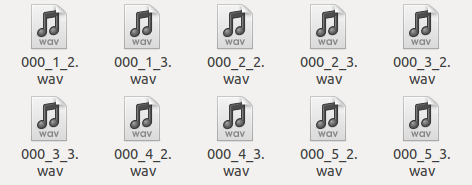
\includegraphics[width=0.7\linewidth]{images/voiceSamples.png}
  \caption{Exemple des fichiers correspondants à l'utilisateur avec l'identifiant \textbf{000}}
\end{figure}

Cela nous permet de disposer de 1060 fichiers audio au total, dont la moitié sera utilisée pour ce projet.

Nous avons donc 530 échantillons de voix, que nous allons alors diviser en 2 :
\begin{itemize}
  \item les enregistrements où des chiffres sont répétés seront utilisés pour \textbf{entraîner} nos modèles
  \item les enregistrements où une phrase est dites seront utilisés pour \textbf{tester} nos modèles
\end{itemize}

\subsection{Extraction des caractéristiques des données}
L'extraction des paramètres spectraux des signaux sonores consiste à obtenir les vecteurs acoustiques stockés dans des fichiers .prm. Nous avons opter d'utiliser mfcc avec 20 coefficients cepstrales. Spro fournit la commande "sfbcep" basée sur filter-bank. Cette commande prend en entrée un signal et sort un fichier de données FBCEPSTRA SPro. Pour chaque trame du signal, une analyse de filter-bank est effectuée et une transformée en cosinus discrète est appliquée à la sortie. Les vecteurs  sont calculés toutes les 10 ms en utilisant une fenêtre d'analyse se chevauchant de 25 ms.

\subsection{Normalisation des caractéristiques}

La normalisation est une technique souvent appliquée dans le cadre de la préparation des données pour l'apprentissage automatique. Le but de la normalisation est de changer les valeurs des colonnes numériques de l'ensemble de données à une échelle commune, sans fausser les différences dans les plages de valeurs. Dans notre cas le volume (  amplitude ) des enregistrements peut varier , on peut avoir un enregistrement avec une voix haute ou à voix faible ainsi il est nécessaire de faire une normalisation.

Le résultat de cette étape nous permet d'avoir des nouveaux fichiers .norm.prm que l'on va stocker dans les mêmes répertoires prm ainsi que des fichiers d'étiquettes indiquant l'étiquette temporelle des trames vocales dans ./data/lbl/

\subsection{Entraînement des modèles}

À l'aide des outils disponibles avec ALIZÉ, nous allons pouvoir créer des modèles correspondants à nos locuteurs. Ces modèles seront utilisés par la suite pour effectuer des comparaisons entre différentes voix et déterminer l'identité des personnes à qui elles appartiennent. Il est à noté qu'entraîner les modèles nécessaires pour ce genre de projet nécessite une certaines puissance de calcul, et que plus nous avons de données à traiter, plus ce calcul sera long.

\subsubsection{Modèle du monde}

Tout d'abord, nous allons créer un modèle de locuteur \textit{général}. Cette étape nous permettra de générer un modèle universel (\textit{Universal Background Model)}, qui nous permettra d'obtenir une représentation des caractéristiques qui forment la parole. Ce dernier est entraîné en utilisant l'ensemble des fichiers correspondants aux locuteurs dont nous disposons. 

Nous utilisons le programme \guillemotleft{}~TrainWorld~\guillemotright{}, présent dans ALIZÉ / \texttt{LIA\_RAL}, afin de créer ce modèle.

\subsubsection{Modèle pour chaque locuteur}

Nous allons maintenant pouvoir entraîner les modèles correspondants à chaque locuteur dont nous voudrons vérifier l'identité par la suite.
Chacun d'eux sera généré en utilisant le modèle du monde crée précédemment, ainsi que les fichiers correspondants au locuteur pour lequel le modèle sera produit.

Comme dit dans la section~\ref{data-split}, page~\pageref{data-split} \guillemotleft{}~\textbf{Données utilisées}~\guillemotright{}, les fichiers utilisés pour entraîner le modèle d'une personne seront ceux dans lesquels elle dit des chiffres.

Nous pouvons utiliser le programme \guillemotleft{}~TrainTarget~\guillemotright{}, qui va générer les modèles correspondants à chaque locuteur.\\
Avant cela, nous devons lui fournir un fichier \guillemotleft{}~.ndx~\guillemotright{}, dans lequel chaque ligne contient le nom du modèle du locuteur qui sera généré, suivi des noms des fichiers vocaux à utiliser pour son entraînement. Pour créer et remplir ce fichier avec les informations qui nous intéressent, nous avons écrit un script (en bash) qui nous permet d'automatiser sa génération, et lui fournit toutes les données qui lui sont nécessaires.

\begin{figure}[htbp]
  \centering
  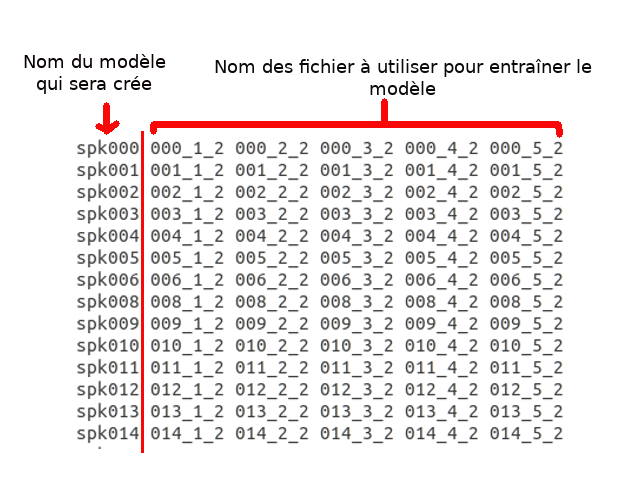
\includegraphics[width=1\linewidth]{images/trainFile.png}
  \caption{Fichier contenant les informations nécessaires à l'entraînement des modèles de locuteur. Le modèle \textbf{spk000} correspond au 1er locuteur, et se servira des fichiers lui correspondant (ceux commençant par \textbf{000})}
\end{figure}

Nous faisons en sorte que chaque modèle qui sera crée utilise les 5 enregistrements de voix 

\subsection{Test des modèles}

Une fois les modèles de chaque locuteur entraînés, il convient de les tester, afin de déterminer leur performance et la justesse des résultats produits. Ici encore, ALIZÉ nous donne accès à des outils permettant de réaliser ces tests. Il s'agit en l'occurrence du programme \guillemotleft{}~ComputTest~\guillemotright{}. Ce dernier va utiliser les modèles des locuteurs et les comparer avec des échantillons de voix de test, afin de générer des scores correspondant au taux de probabilité que les 2 appartiennent à la même personne.

Ce programme nécessite lui aussi un fichier de configuration de type \guillemotleft{}~.ndx~\guillemotright{}. Nous allons, là aussi, automatiser sa création à l'aide d'un script.\\

En pratique, ce fichier contient la liste des noms de fichiers de test (comme présenté dans la section~\ref{data-split}, page~\pageref{data-split}, il s'agira ici des enregistrements audio où les locuteurs disent des phrases complètes), suivis des noms des modèles de locuteurs précédemment entraînés, et que nous voulons tester.

\begin{figure}[htbp]
  \centering
  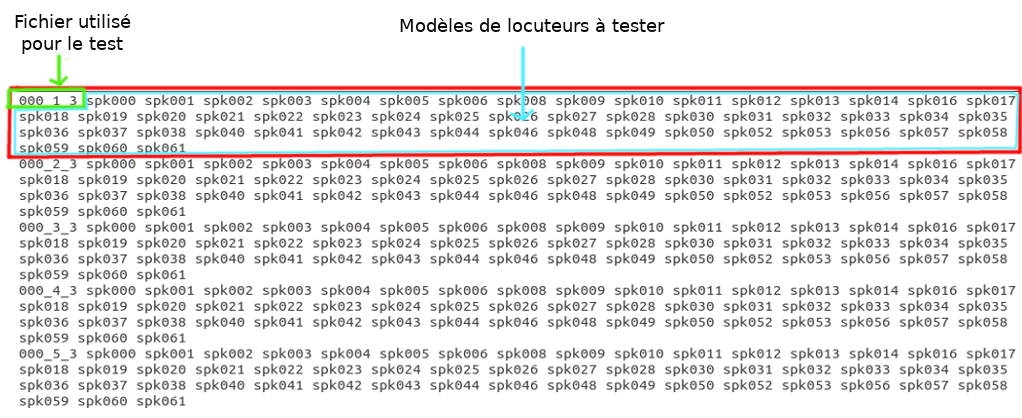
\includegraphics[width=1\linewidth]{images/testFile.png}
  \caption{Fichier contenant les informations nécessaires au test des modèles crées}
\end{figure}

Dans notre cas, nous souhaitons tester tous les fichiers de test dont nous disposons, avec tous les modèles de locuteurs qui ont été entraînés.

\subsection{Interprétation des résultats obtenus}

La phase de test nous permet donc d'obtenir des résultats qui nous permettrons de savoir si notre programme réussi à identifier des locuteurs, mais aussi de connaître son niveau de précision, le taux d'erreurs, etc.\\

À l'issue de l'étape précédent, notre programme à généré un fichier contenant des résultats, qu'il nous reste à analyser. 

Ces derniers sont représentés sous une forme de liste, où chaque ligne correspond à un test entre un modèle de locuteur et un échantillon audio. Ces ligne se décomposent comme suit :

\begin{itemize}
  \item la 1ère colonne correspond au sexe du locuteur (non utilisé dans ce projet) 
  \item la 2ème nous informe sur le nom du modèle testé
  \item la 3ème indique si le score est négatif (0) ou positif (1)
  \item la 4ème correspond au nom du fichier de test
  \item enfin, la dernière n'est autre que le score obtenu
\end{itemize}

\begin{figure}[htbp]
  \centering
  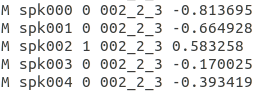
\includegraphics[width=0.5\linewidth]{images/goodResultExample.png}
  \caption{Exemple de fichier contenant les résultats des tests}
\end{figure}
 

\subsection{Identification du locuteur}

Afin de pouvoir dire avec fiabilité si un locuteur à bien été identifié, il est nécessaire d'analyser les résultats obtenus à l'issue des étapes précédentes. Nous nous intéressons au score affiché en fin de chaque ligne du fichier de résultat, et voulons notamment savoir à partir de quelle valeur nous pouvions considérer que ce dernier représentait une identification positive. Nous avons obtenu un total de 14045 comparaisons.

Dans un premier temps, il est possible de filtrer ces résultats selon le signe du score (positif ou négatif), puisque les scores négatifs présents dans notre document signifient dans la majorité des cas que la voix du locuteur (modèle) ne correspond pas à celle testée, et qu'il s'agit donc de 2 personnes différentes. Il nous reste ainsi 1479 résultats où le score est positif.

En ne conservant que ces scores, nous pouvons alors réduire le nombre de résultats à traiter.

Dans un second temps, nous pouvons analyser les résultats restants afin de définir à partir de quel score les locuteurs sont correctement identifiés. Il se trouve que les scores supérieurs à 0.4 permettent une identification correcte du locuteur dans une majorité des cas, néanmoins, nous observons des erreurs d'identifications. Dans ce cas, nous pouvons augmenter la valeur du score considéré comme acceptable (à 0.5 par exemple), et ainsi réduire le nombre de faux positifs.

\begin{figure}[htbp]
  \centering
  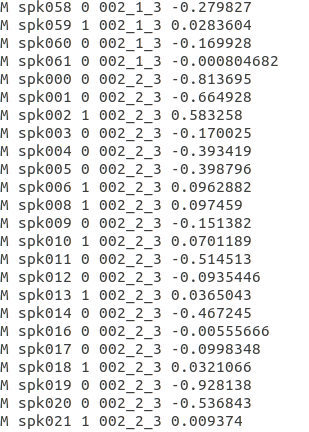
\includegraphics[width=0.5\linewidth]{images/badResultExample.png}
  \caption{Résultat de plusieurs tests. Ici le locuteur \textbf{spk002} est correctement identifié (score de 0.58), tandis que les autres ont soit un score négatif soit trop faible, et ne sont donc pas pris en considération}
\end{figure}

% chapitre 5 : Conclusion et perspectives

\chapter{Conclusion et Perspectives\label{chap-conclusion}}

Avant d'entamer le travail sur ce projet nous n'avions pas forcément toutes les connaissances nécessaires au développement d'outils dans ce genre de domaine.
Mais au fur et à mesure, nous avons eu l'opportunité d'étudier les outils, techniques, méthodes, etc, nécessaires à un tel travail.
De plus, nous avons pu voir les différents domaines et les différentes plateformes sur lesquels la reconnaissance de la parole était utilisée, ce qui nous à permis de visualiser les opportunités possibles, tant sur un plan professionnel que de simple curiosité personnelle.\\

Aussi, une fois le programme réalisé, nous avons pu analyser les résultats produits et déterminer qu'ils étaient grandement améliorables.\\

Ces améliorations pourraient être apportées sur de prochains travaux de ce type, notamment au niveau de la réflexion quant aux outils ou techniques utilisés, qui offrent des possibilités très vastes, dont nous aurions pu tirer un peu plus parti. De plus, des considérations quant a la plateforme d'utilisation du programme pourraient être intéressantes, puisque ALIZÉ dispose par exemple d'outils permettant son utilisation su système Android.

\begin{thebibliography}{9}
\bibitem{tp-exemple} 
D. Istrate.
\textit{TP Biométrie : Reconnaissance du locuteur}. 
ESIGETEL.

\bibitem{gmm} 
Iosif Mporas, Todor Ganchev, Mihalis Siafarikas, Nikos Fakotakis
\textit{Comparison of Speech Features on the Speech Recognition Task}. 
Department of Electrical and Computer Engineering, University of Patras 26500 Rion-Patras, Greece, Journal of Computer Science 3 (8): 608-616, 2007

\bibitem{article2} 
Jonathan Hui.
\textit{Speech Recognition - GMM, HMM}.
[\textit{\texttt{https://medium.com/@jonathan\_hui/speech-recognition-gmm-hmm-8bb5eff8b196}}].
Medium, sep 2019.

\bibitem{spro-0}
Site web officiel du projet SPro.
\textit{http://www.irisa.fr/metiss/guig/spro}.

\bibitem{spro-doc}
Documentation en ligne pour SPro.
\textit{https://www.irisa.fr/metiss/guig/spro/spro-4.0.1/spro.html}.

\bibitem{alize.0}
Site web officiel du projet ALIZÉ.
\textit{https://alize.univ-avignon.fr}.

\bibitem{alize-1} 
Aurelien Mayoue. 
\textit{Reference System based on speech modality}. 
GET-INT, 2006-2007.

\bibitem{alize-2} 
Aitor Hernández López. 
\textit{Evaluation of the ALIZE/\texttt{LIA\_RAL} Speaker Verifcation Toolkit on an Embedded System}. 
University Of Computer Science of Vienna (ICT), feb 2015.

\bibitem{alize-3} 
Anthony Larcher, Jean-François Bonastre, Benoît Fauve, Kong Aik Lee, Christophe Levy, Haizhou Li, John Mason, Jean-Yves Parfait.
\textit{ALIZE 3.0-Open Source Toolkit for State-of-the-Art Speaker Recognition}. 
Annual Conference of the International Speech Communication Association, Aug 2013, Lyon, France.
\end{thebibliography}

%\bibliographystyle{alpha}
%\bibliography{memoire}
\end{document}
